\section{Results}

\subsection{Step-by-step Example with OR}
Recall the two bit function OR which returns $1$ if there
is at least a single $1$ in the input and returns $0$ otherwise.
To understand Reichardt's formulation and the conversion
to Boyd's standard form, consider as inputs to our tool
the case with function $f: D \rightarrow E$ where
$D \subseteq {\{0,1\}}^2$ and $E =\{OR(x): x \in D \}$.
Let $F$ be the set of $(y,z)$ such that $f(y) \neq f(z)$. In this
case, $F = \{(00,01), (00,10), (00,11), (01,00), (10,00), (11,00)\}$

Our matrix $\X$ will be created as follows:
\begin{align}
\X = \begin{blockarray}{ccccc}
\qquad & 00 & 01 & 10 & 11 \\
\begin{block}{c[cccc]}
  00 & X_{(00,00)} & X_{(00,01)} & X_{(00,10)} & X_{(00,11)}\\
  01 & X_{(01,00)} & X_{(01,01)} & X_{(01,10)} & X_{(01,11)}\\
  10 & X_{(10,00)} & X_{(10,01)} & X_{(10,10)} & X_{(10,11)}\\
  11 & X_{(11,00)} & X_{(11,01)} & X_{(11,10)} & X_{(11,11)}\\
\end{block}
\end{blockarray} \nonumber 
\end{align}


The objective function of the SDP is:
\begin{align} \label{eq:reichardtObj} 
    f_{\text{bound}} &= M(\X) = \max_{y \in D} \sum_{j \in [n]}
    \bra{y,j}\X\ket{y,j} \nonumber \\
    &= \max\{ \tr{X_{(00,00)}}, \tr{X_{(01,01)}}, \tr{X_{(10,10)}}, \tr{X_{(11,11)}} \} \nonumber
\end{align}
subject to constraints
\begin{align}
    \X \succcurlyeq 0  \nonumber 
\end{align}
and
\begin{align}
    \forall (y,z) \in F \sum_{j \in [n]: y_j \ne z_j} 
    \bra{y,j} \X \ket{z, j} = 1. \nonumber 
\end{align}
Which is equivalent to:
\begin{align}
    \tr{X_{(00,01)}} &= \tr{X_{(00,10)}} = \tr{X_{(00,11)}} = 1 \nonumber \\
    \tr{X_{(01,00)}} &= \tr{X_{(10,00)}} = \tr{X_{(11,00)}} = 1 \nonumber
\end{align}

Our goal is to minimize $M$, and thus $f_{\text{bound}}$ by finding the optimal value of $\X$. By running our SDP solver, we obtain $\X$ with an objective function value of $\sqrt{2}$.
\begin{align}
    \X = \left[ \begin{array}{cc|cc|cc|cc}
    0.7 & 0 & 0 & 0 & 1 & 0 & 0.5 & 0\\
    0 & 0.7 & 0 & 1 & 0 & 0 & 0 & 0.5\\
    \hline
    0 & 0 & 0 & 0 & 0 & 0 & 0 & 0\\
    0 & 1 & 0 & \sqrt{2} & 0 & 0 & 0 & 0.7\\
    \hline
    1 & 0 & 0 & 0 & \sqrt{2} & 0 & 0.7 & 0\\
    0 & 0 & 0 & 0 & 0 & 0 & 0 & 0\\
    \hline
    0.5 & 0 & 0 & 0 & 0.7 & 0 & 0.6 & 0\\
    0 & 0.5 & 0 & 0.7 & 0 & 0 & 0 & 0.6\\
    \end{array}
\right] \nonumber
\end{align}

The columns of this matrix are the vectors used in the span program 

We then use this to obtain $L$ where $L^\dagger L = \X$. From here we can then obtain $\bra{v_{x,i}}$ for all $x \in D$, $i \in [n]$. Then using the definition of $I$ from earlier:

\begin{align}
I &= \left[\begin{array}{cc}
    \bra{1}\bra{v_{00,1}} & \bra{1}\bra{v_{00,2}} \\
    \bra{1}\bra{v_{01,1}} & \bra{0}\bra{v_{01,2}} \\
    \bra{0}\bra{v_{10,1}} & \bra{1}\bra{v_{10,2}}\\
    \bra{0}\bra{v_{11,1}} & \bra{0}\bra{v_{11,2}}\\
\end{array} \right] \nonumber \\
&= \left[\begin{array}{c|c|c|c}
    0 \cdots 0 & \bra{v_{00,1}} & 0 \cdots 0 & \bra{v_{00,2}} \\
    0 \cdots 0 & \bra{v_{01,1}} & \bra{v_{01,2}} & 0 \cdots 0\\
    \bra{v_{10,1}} & 0 \cdots 0 & 0 \cdots 0 & \bra{v_{10,2}}\\
    \bra{v_{11,1}} & 0 \cdots 0 & \bra{v_{11,2}} & 0 \cdots 0\\
\end{array} \right] \nonumber
\end{align}

The columns of this matrix are the columns used in the span program. If we remove rows of $I$ corresponding to elements $ x \in D$ such that $f(x) = 1$, and columns of $I$ that are the all zero vector, we obtain an equivalent $I$:

\begin{align}
I &= \left[\begin{array}{c|c|c|c}
   0 & 1 & 0 & 1 \\
\end{array} \right] \nonumber \\
\tau &= 1 \nonumber
\end{align}

In both definitions of $I$ the left two partitions correspond to the first bit in the
input, and the right two partitions correspond to the second bit of the input. For each
input bit, the relevant block of $I$ is broken into left and right halves, corresponding
to whether the bit is $0$ or $1$ respectively. It is clear from this matrix that if either input bit is $1$ the function will evaluate to True, and otherwise evaluate to False.

\begin{figure}[ht]
\centering
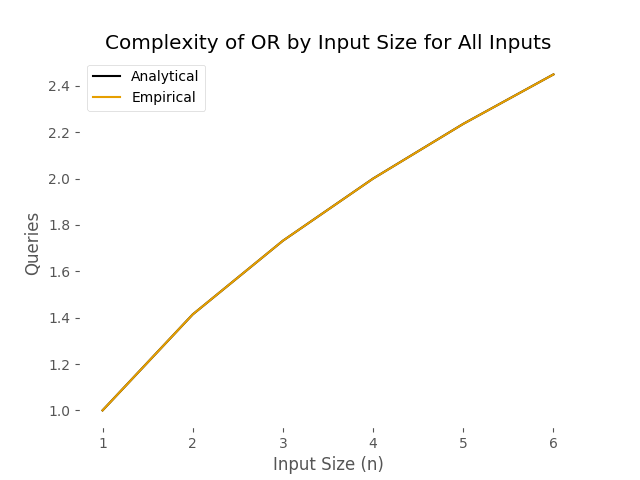
\includegraphics[scale=.5]{figures/or_all_complexity.png}
\caption{The proven analytical optimal query complexity
and calculated empirical optimal query complexity by 
size of input bit string.}
\label{fig:or_all_complexity}
\end{figure}

\begin{figure}[ht]
\centering
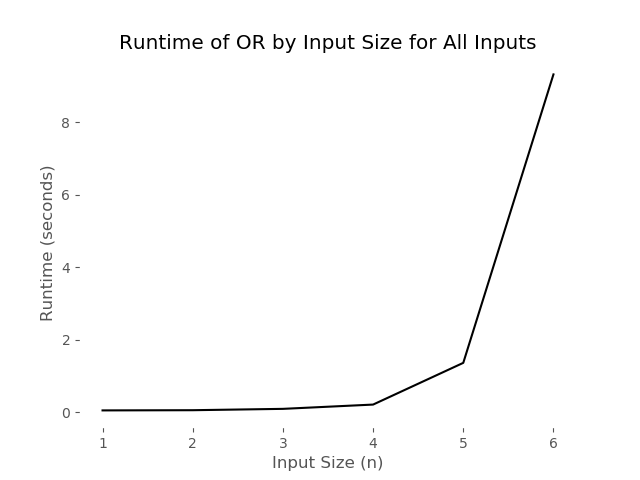
\includegraphics[scale=.4]{figures/or_all_runtime.png}
\caption{runtime of SDP solver by size of input strings.}
\label{fig:or_all_runtime}
\end{figure}

\subsection{OR Function: Worst-case Boolean Inputs}\label{sec:speed}
In \cref{fig:or_all_complexity}, observe that our algorithm
correctly calculates the optimal query complexity of the OR function (the
analytical and empirical lines are so close that one
is mostly obscured).
Our algorithm's performance is displayed in \cref{fig:or_all_runtime}.
We see that runtime grows exponentially with respect to input size as expected, 
given the exponential increase in the cardinality of the set $D$ of all
inputs of length $n$. 
We also see that our algorithm is accurately calculating the
optimal quantum query complexity of the OR function. 

The correctness of our algorithm is supported by it's performance on the OR function as it exactly matches the theoretical values. This is further supported by the proofs of Reichardt, Wen, and our Methodology section. In addition, we have made our source code available on GitHub for review. Given the correctness of our algorithm, we can address improvements to its runtime.

First, we can attempt to improve runtime while
maintaining the correctness of the algorithm. Later,
we might be able to alter the algorithm
mathematically to take advantage of the structure
given in SDP's formed from quantum algorithms. 
It has also been claimed that the dual of this semidefinite
programming problem yields the quantum algorithm with minimal query complexity.
However, this optimal solution to the dual may not be easily 
interpreted as an algorithm as there could be many optimal, feasible solutions. 
Semidefinite programming problems also don't guarantee the tightness of the dual,
as is the case in linear programming. 
These problems all pose potential areas of future expansion.

\subsection{OR Function: All Boolean Inputs}

A simple approach to speeding up the runtime of our
algorithm is to simply decrease the number of input
strings considered for a given input size $n$. It's
important that we still obtain a good approximation
of the correct answer, so we need to ensure that the
inputs we do analyze will lead to the correct result.
Because the bounds of our algorithm are adversarial,
meaning that they are worst-case bounds, we can opt
to only use the worst-case inputs.

Again returning to our OR example, the hardest inputs are
either entirely zeros, or contain only a single 1. 
Using these inputs, we can then run our algorithm to 
compare both runtime and precision of results.

\begin{figure}[ht]
\centering
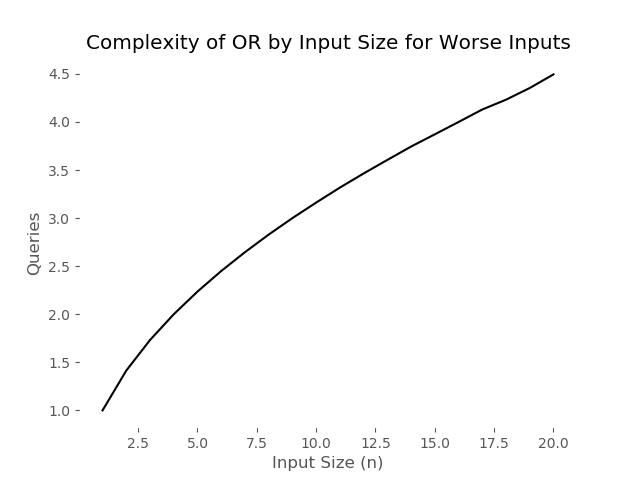
\includegraphics[scale=.5]{figures/or_worst_complexity.png}
\caption{The proven analytical optimal query complexity
and calculated empirical optimal query complexity by 
size of input bit string.}
\label{fig:or_worst_complexity}
\end{figure}

\begin{figure}[ht]
\centering
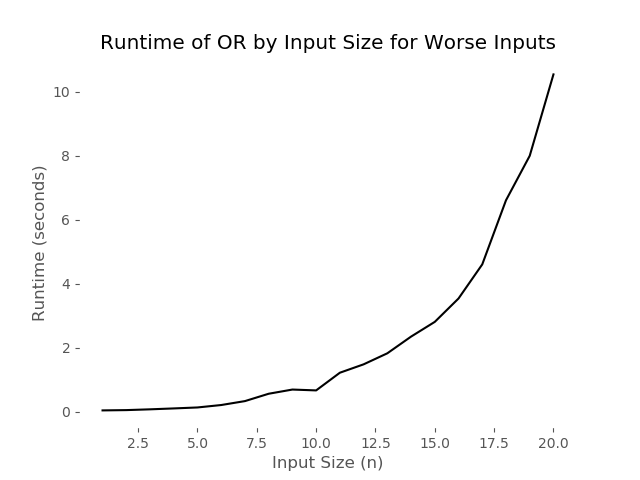
\includegraphics[scale=.4]{figures/or_worst_runtime.png}
\caption{Runtime of SDP solver by size of input strings.}
\label{fig:or_worst_runtime}
\end{figure}

The runtime is drastically improved over the all-case scenario. 
This result is not only shown via \todo{put both runtimes on the same figure and reference it here} of the graphs, 
but also in the x-axis because the speed up was so 
significant that we were able to solve for many more 
input sizes than in the all-case scenario. 
Looking at the optimal query complexities returned, 
we observe that we are still obtaining good 
approximations of the true value. 
We believe that more iterations could drastically 
improve the performance of the algorithm as well as 
improved stopping conditions. Instead of simply stopping 
after some number of iterations (in this case 100), 
we could look to see if the improvements to the objective 
function are negligible and conclude that the algorithm has converged.
